\section{Ομαδοποίηση χρηστών}
\subsection{Προεπεξεργασία των δεδομένων}
Τα δεδομένα όπως παρέχονται από το dataset, στη μορφή όπου κάθε γραμμή αποτελεί μία βαθμολογία ενός χρήστη σε μία ταινία, δεν είναι ικανά για να ομαδοποιήσουν τους χρήστες βάσει των προτιμήσεων τους και πρέπει πρώτα να επεξεργαστούν.
Εφόσον θέλουμε να ομαδοποιήσουμε χρήστες και όχι βαθμολογίες, πρέπει να αναπαραστήσουμε κάθε χρήστη ως ένα διάνυσμα χαρακτηριστικών που να εκφράζουν την προτίμησή του σε ταινίες.
Ένας απλός τρόπος θα ήταν να μοντελοποιήσουμε κάθε χρήστη ως ένα διάνυσμα διάστασης 1682, όσες είναι και οι ταινίες όπου το κάθε στοιχείο είναι η βαθμολογία του για τη συγκεκριμένη ταινία ή 0 αν δεν την έχει βαθμολογήσει.
Εύκολα μπορεί να δει κανείς ότι αυτή η μοντελοποίηση καταλήγει σε πολύ μεγάλο και υπολογιστικά αποκρουστικό πίνακα δεδομένων αφού η διάσταση κάθε χαρακτηριστικού είναι 1682, και επίσης αυτός ο πίνακας θα είχε πολλά μηδενικά όπου δε προσφέρουν πληροφορία.

Από μία άλλη οπτική γωνία αντί για τον χώρο των ταινιών να αναπαρασταθούν στο χώρο των κατηγοριών ταινιών, δηλαδή το διάνυσμα του χρήστη να είναι διάστασης 18, όσες είναι και οι κατηγορίες των ταινιών και κάθε στοιχείο να ποσοτικοποιεί με κάποιο τρόπο τη προτίμηση του χρήστη για τη συγκεκριμένη κατηγορία.
Ένας τρόπος είναι να αθροίσουμε όλες τις βαθμολογίες του χρήστη για τη συγκεκριμένη κατηγορία και όπου η βαθμολογία είναι 1 ή 2 στα 5 να μετράει αρνητικά.
Όμως έτσι δύο χρήστες που έχουν αναλογικά τις ίδιες προτιμήσεις κατηγοριών, θα έχουν μεγάλη απόσταση (με οποιοδήποτε μέτρο) αν ο ένας έχει δει λίγες ταινίες και ο άλλος πολλές.
Πχ έστω user1 = [10 30 50], user2 =  [105 310 490] user3 = [40 -10 -20] οι προτιμήσεις τριών χρηστών για τρεις κατηγορίες ταινιών.
Παρατηρούμε ότι και για τους δύο πρώτους τους αρέσει περισσότερο η τρίτη μετά η δεύτερη και μετά η πρώτη κατηγορία, αλλά η απόσταση του user1 με τον user2 είναι πολύ μεγαλύτερη από την απόσταση μεταξύ του user1 και user3 επειδή διαφέρουν στο πλήθος των βαθμολογήσεων που έχουν κάνει! Ευτυχώς το μειονέκτημα αυτό διορθώνεται εύκολα ομαλοποιώντας τα αθροίσματα αυτά διαιρώντας με το πλήθος των βαθμολογήσεων και τελικά καταλήγουμε στην αναπαράσταση του χρήστη με τους μέσους όρους των βαθμολογιών του στις ταινίες της αντίστοιχης κατηγορίας.
Δηλαδή κάθε χρήστης αποτελείται από ένα 18-διάστατο διάνυσμα όπου το κάθε στοιχείο βρίσκεται στο εύρος [1\ldots5] των πραγματικών αριθμών.
Όπου κάποιος χρήστης δεν έχει βαθμολογήσει καμία ταινία μιας κατηγορίας, τοποθετούμε τη μέση τιμή της αντίστοιχης κατηγορίας εξαιρώντας τις υπόλοιπες κενές τιμές.

\subsection{Εκτίμηση πλήθους των ομάδων}
Για να εκτιμήσουμε το πλήθος των ομάδων των χρηστών χρησιμοποιούμε τον βασικό ακολουθιακό αλγόριθμο ομαδοποίησης (BSAS) χρησιμοποιώντας ως μέτρο ανομοιότητας μεταξύ δύο διανυσμάτων χαρακτηριστικών την ευκλείδεια απόσταση τους και βάζοντας ως μέγιστο αριθμό ομάδων Q έναν μη περιοριστικό αριθμό (πχ όσοι είναι οι χρήστες, Ν).
Αρχικά διαλέγουμε 60 τιμές από ένα ικανοποιητικό εύρος για το κατώφλι απόστασης Θ και έπειτα εφαρμόζουμε τον αλγόριθμο 7 φορές για κάθε τιμή του Θ.
Για κάθε τιμή Θ διαλέγουμε από τα 7 αποτελέσματα το πιο συχνά εμφανιζόμενο πλήθος ομάδων και κάνουμε την αντίστοιχη γραφική παράσταση τους.

\clearpage
\begin{figure}[ht]
	\makebox[\textwidth][c]{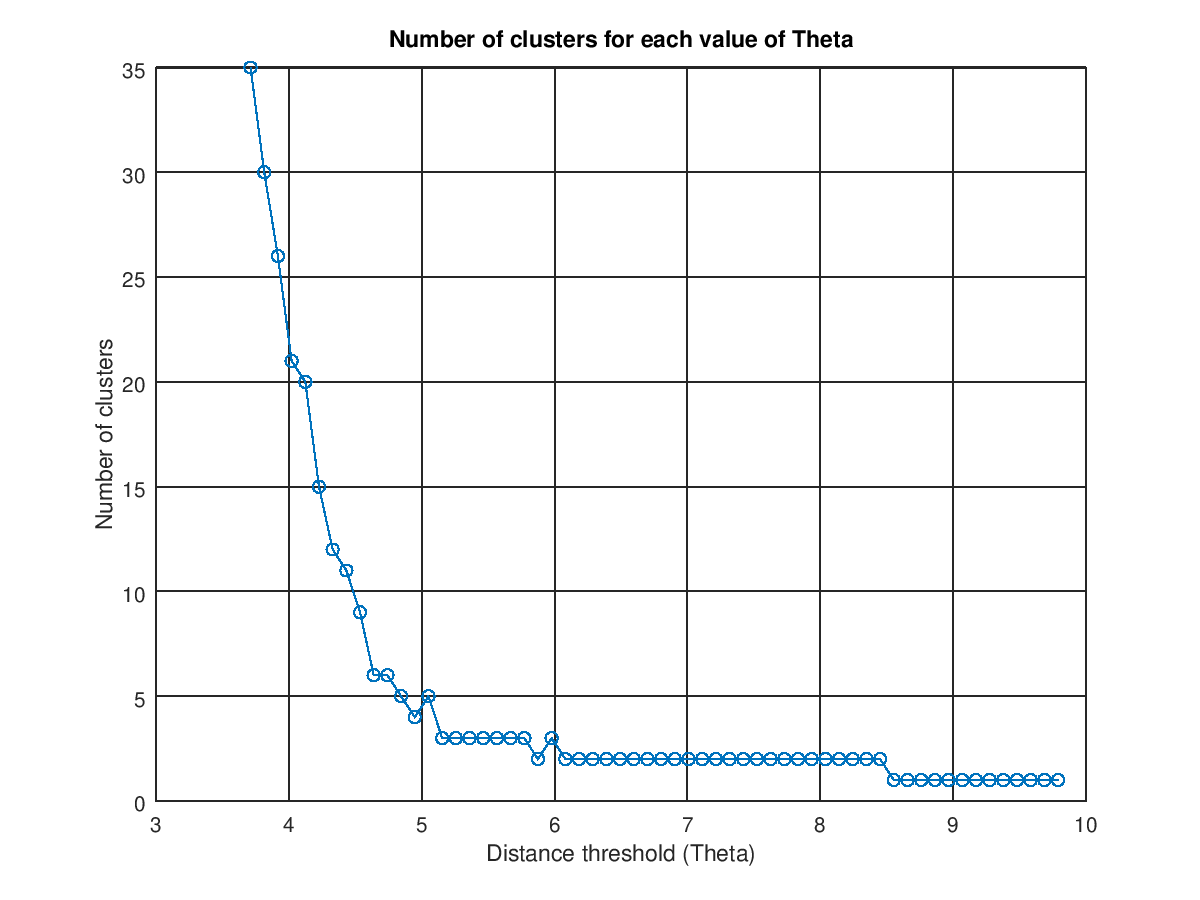
\includegraphics[width=1.35\textwidth]{theta_v_clust.png}}
\end{figure}

Από το σχήμα παρατηρούμε ότι το πιο συχνά εμφανιζόμενο πλήθος ομάδων είναι 2 και επιλέγεται αυτό, ενώ στη δεύτερη θέση βρίσκεται το 3.
Επίσης παρατηρούμε μερικά σκαμπανεβάσματα που δικαιολογούν την ευαισθησία του αλγορίθμου BSAS στην σειρά εμφάνισης των δεδομένων.

\subsection{Εφαρμογή του αλγορίθμου K-means}

Κατά την εκτίμηση του πλήθους των ομάδων χρησιμοποιήσαμε τον αλγόριθμο BSAS ο οποίος εκτός από το πλήθος των ομάδων βρίσκει και μια ομαδοποίηση των χρηστών που συνήθως δεν είναι τόσο ικανοποιητική.
Στη συνέχεια εφαρμόζουμε ακόμα 2 αλγορίθμους ομαδοποίησης, k-means  και μια απλή εκδοχή του βασικού ιεραρχικού συσσωρευτικού σχήματος (GAS).
Προκειμένου να εφαρμόσουμε τον k-means θέτουμε το πλήθος ομάδων ίσο με 2 και αρχικοποιούμε τα κεντροειδή ως τυχαία ομοιόμορφα διανύσματα στο υποσύνολο [1,5] του \(R^{18}\).
Για την προβολή των αποτελεσμάτων χρησιμοποιούμε την συνάρτηση parallelcoords (η οποία βρίσκεται μόνο στο matlab αλλά την υλοποιήσαμε πρόχειρα για συμβατότητα με το octave).

\begin{figure}[h]
	\makebox[\textwidth][c]{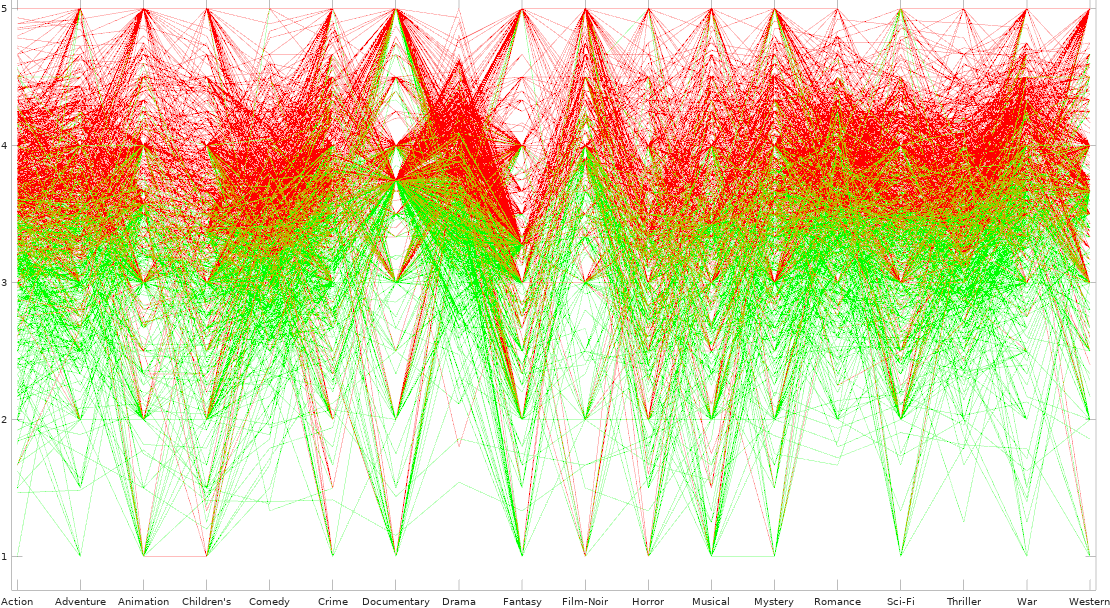
\includegraphics[width=1.455\textwidth]{kmeans_parallel.png}}
\end{figure}

Παρατηρούμε ότι χρήστες της κόκκινης ομάδας βρίσκονται γενικά πιο πάνω από αυτούς στη πράσινη ομάδα για τις περισσότερες κατηγορίες.
Οπότε συμπεραίνουμε ότι η ομαδοποίηση αυτή χωρίζει τους χρήστες σε γενικά \textit{γενναιόδωρους} και \textit{τσιγκούνηδες} ως προς τις βαθμολογίες που έχουν κάνει.

\subsection{Εφαρμογή του συσσωρευτικού αλγορίθμου πλήρους δεσμού}
Έπειτα εφαρμόζουμε τον συσσωρευτικό αλγόριθμο πλήρους δεσμού, ο οποίος ως ένας ιεραρχικός αλγόριθμος σε αντίθεση με τους προηγούμενους αλγορίθμους παράγει πολλές ομαδοποιήσεις των δεδομένων.
Στην αρχή ξεκινάει με \(N\) ομάδες και σε κάθε βήμα ενώνει τις 2 πιο κοντινές ομάδες και ανανεώνει τις αποστάσεις με βάση το κριτήριο πλήρους δεσμού που σημαίνει ότι μετά από κάθε ενοποίηση η απόσταση μεταξύ της καινούργιας ομάδας \(C_q = C_i \cup C_j\) με κάθε παλιά ομάδα \(C_k\) είναι η μέγιστη μεταξύ της \(C_k\) με τις \(C_i\) και \(C_j\).
Οι αρχικές αποστάσεις μεταξύ των διανυσμάτων ορίζονται ως η ευκλείδεια απόσταση τους και αποθηκεύονται σε ένα πίνακα εγγύτητας.

Μπορούμε να δούμε όλες τις ομαδοποιήσεις κατευθείαν από το πίνακα bel που επιστρέφει ο agglom(\dots) όπου οι γραμμές αναπαριστούν τις ομαδοποιήσεις που προέκυψαν με τη σειρά.
Αλλά αυτός ο τρόπος είναι δύσχρηστος και όχι τόσο όμορφος, γι’ αυτό το λόγο τις αναπαριστούμε χρησιμοποιώντας δενδρόγραμμα, με τη dendrogram(\dots) που προϋποθέτει όμως η είσοδος να είναι της μορφής που δίνει η linkage(\dots) η οποία υλοποιεί μια γκάμα από αλγορίθμους αυτού του είδους (απλού δεσμού, πλήρους δεσμού κτλπ).


\begin{figure}[h]
	\makebox[\textwidth][c]{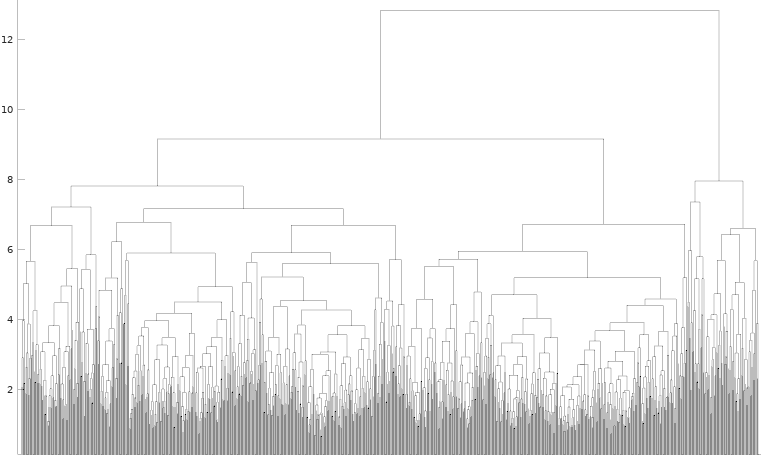
\includegraphics[width=1.182\textwidth]{agglom.png}}
\end{figure}

Σε αυτήν την εικόνα βλέπουμε τις ομαδοποιήσεις πλήρους δεσμού που περιγράψαμε πιο πάνω.
Στην αρχή ο κάθε χρήστης είναι μια ομάδα μόνος του και όσο ανεβαίνουμε επίπεδο οι ομάδες συγχωνεύονται κατάλληλα, οδηγώντας τελικά σε μια ομάδα.
Σε απόσταση \(\sim 9\) υπάρχουν δυο ομάδες, όπως είχαμε βρει στους αλγορίθμους BSAS και k-means, ενώ σε απόσταση στο εύρος [7,8] παρατηρούμε 3 με 5 ομάδες.
Αν και ακούγεται πιο σωστό να χωρίσουμε του χρήστες σε αρκετές ομάδες, δεν είναι εύκολο να πούμε με ποια φυσικά κριτήρια χωρίζονται οι χρήστες σε αυτές τις ομάδες.
Θα ήταν καλό να έχουμε έναν λογικό αριθμό ομάδων με αρκετούς χρήστες η κάθε μια.
\textit{Τελικά 2 ή 3 ομάδες είναι ένας καλός αριθμός για να χωρίσουμε τους χρήστες μας στον συσσωρευτικό αλγόριθμο.}
